\section{The ForeC Language}
\label{sec:forecLanguage}

%-----------------------------------------------------------------------------

\subsection{The Synchronous Approach}
Synchronous languages are based on the synchronous hypothesis~\cite{timed_synchronous_survey},
which states that a system reacts instantaneously to environmental
events. Thus, the synchronous hypothesis assumes that the system 
executes infinitely fast, in zero time. This separates the physical 
time of the environment from the execution time of the system, 
which depends on the implementation of the system.
Figure~\ref{fig:synchronous_moc} depicts a synchronous 
program defined as a set of concurrent threads. The threads 
take inputs from the environment, perform their computations,
and then emit their outputs to the environment. 
Concurrent threads can communicate with each other (dashed 
arrows in Figure~\ref{fig:synchronous_moc}) during their
computation. The communication is instantaneous due to 
the synchronous hypothesis. A synchronous program 
can be thought of as being driven by a hypothetical (logical) \emph{global clock}
that discretises the program's execution. The speed 
of the global clock is determined by the system's specifications. 
When a thread completes its computation, we say that the thread 
has completed its \emph{local} tick. When all threads in the 
program have completed their local tick, we say that the program
has completed its \emph{global} tick. 
The separation of physical time from execution time simplifies 
the language semantics and enables formal verification. Once the 
system is implemented, it is necessary to verify the synchronous 
hypothesis. That is, the Worst-Case Execution Time (WCET) of each 
global tick must not exceed the specified period (in physical time) 
of the global clock.

\begin{figure}
	\centering
	
	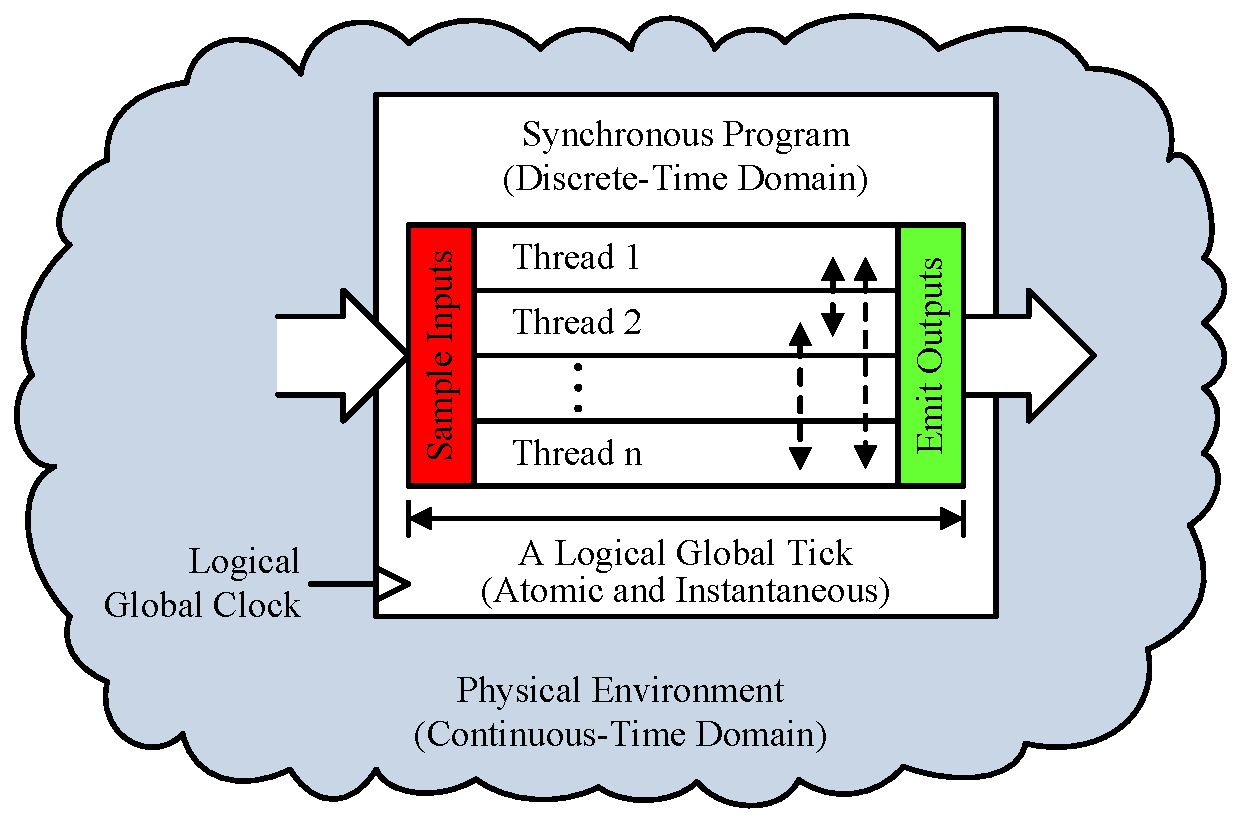
\includegraphics[width=0.6\columnwidth]{synchronous_moc}	
	\caption{Synchronous model of computation.}
	\label{fig:synchronous_moc}
\end{figure}

ForeC extends the C language with synchronous constructs to 
enable the deterministic parallel programming of multicores.
Extending C with synchronous constructs is not new, as the 
following languages demonstrate: Esterel-C Language (ECL~\cite{timed_ecl}), 
\synchronousc{} (SC~\cite{timed_synccharts_c_proposal}), Reactive 
Shared Variables~\cite{timed_reactivec_shared_variables}, 
and \pretc{}~\cite{pret_pretc}. The ECL compiler splits an 
ECL program into an Esterel and a C program. The Esterel program
is compiled in the traditional manner~\cite{timed_compiling_esterel}, 
where the concurrency 
is compiled away, which is unsuitable for multicore execution.
The inherent sequential execution semantics of SC, Reactive C 
and \pretc{} renders them unsuitable for multicore execution. In
contrast, the semantics of ForeC is designed for parallel 
execution on multicores. In particular, ForeC does not impose
a scheduling order on parallel threads. Parallel threads can
be scheduled in an arbitrary order without altering the program's 
behaviour. This scheduling independence is maintained even 
when threads communicate using shared variables. Thus, 
the scheduling of ForeC threads remains flexible and allows 
implementations to balance high execution 
performance against time-predictable execution. The 
remainder of this section details the syntax and semantics 
of the ForeC synchronous constructs.


%-----------------------------------------------------------------------------

\subsection{The ForeC Language Constructs}
ForeC extends C with additional instructions and type-qualifiers.
Figure~\ref{fig:forec_syntax} gives the extended syntax and 
Table~\ref{table:forec_semantics} summarises their semantics.  
A ForeC instruction can be either a classical C instruction or
a block within '\verb${$' and '\verb$}$' (\verb$c_inst$), a
barrier synchronisation (\verb$pause$), an encapsulated fork/join
(\verb$par$), or hierarchical preemption (\verb$abort$). ForeC
variables are declared like in C with a type and type qualifier, 
which can be a C type qualifier (\verb$c_tq$), a qualifier to 
denote variables that are updated by the environment (\verb$input$), a 
qualifier to denote variables that are emitted to the
environment (\verb$output$), or a qualifier to denote variables
that are shared between threads (\verb$shared$). We continue by 
describing each ForeC construct in detail.

\begin{figure}[t]
	\centering

	\renewcommand{\arraystretch}{1.25}
	\begin{tabular}{l r l}
		Instructions:		& \emph{inst} & ::= \emph{c\_inst}																\\
							&			& ~~~| \verb$pause$ | \verb$par($\emph{inst}(,~\emph{inst})*\verb$)$				\\
							&			& ~~~| \verb$weak$?~\verb$abort$~\emph{inst}~\verb$when immediate$?~(\expression{})	\\
																															\\
		Type-Qualifiers:	& \emph{tq}	& ::= \emph{c\_tq}																	\\
							&			& ~~~| \verb$input$ | \verb$output$ | \verb$shared$
	\end{tabular}
	
	\caption{The syntactic extensions to C.}
	\label{fig:forec_syntax}
\end{figure}

\begin{table}[t]
	\centering
	\renewcommand{\arraystretch}{1.25}		

	\begin{tabular}{| p{\textwidth} |}
		\hline
		\textbf{ForeC construct and its Semantics}										\\ 
		\hline
		
		\verb$input$																	\\
			Type-qualifier to declare an input variable, the value of which is updated 
			by the environment at the start of every global tick.						\\ \hline
		\verb$output$																	\\
			Type-qualifier to declare an output variable, the value of which is emitted 
			to the environment at the end of every global tick.							\\ \hline
		\verb$shared$																	\\
			Type-qualifier to declare a shared variable, which can be accessed by 
			multiple threads.															\\ \hline
		\verb$pause$																	\\
			Pauses the executing thread until the next global tick.						\\ \hline
		\verb$par$( \emph{inst} (, \emph{inst})* )										\\
			Forks each instruction \emph{inst} to execute as a parallel thread. The 
			\verb$par$ terminates when all threads have terminated (joined back).		\\ \hline
		\verb$weak$?~\verb$abort$~\emph{inst}~\verb$when immediate$?~(\expression{})	\\
			Preempts its body \emph{inst} when the expression \expression{} evaluates to 
			a non-zero value.															\\
		\hline
	\end{tabular}

	\caption{Semantics of the ForeC constructs.}
	\label{table:forec_semantics}
\end{table}


%-----------------------------------------------------------------------------

\subsubsection{Fork/Join Parallelism}
Like ordinary C programs, the main entry point of a ForeC program
is defined by the \verb$main$ function and serves as the program's
\verb$main$ thread of execution. The ``\verb$par$(\emph{inst}(,~\emph{inst})*)''
instruction is used to \emph{fork} the \verb$main$ thread into parallel 
threads of execution. The \verb$par$ instruction forks its comma-separated 
arguments \emph{inst} to execute as parallel threads. All threads can
use the \verb$par$ instruction to fork their own threads and create
a hierarchy (nesting) of threads. We call the 
thread that executes the \verb$par$ instruction the \emph{parent}
thread, and the threads that are forked the \emph{child} threads.
The \verb$par$ is a blocking instruction that terminates only when all
its child threads have terminated (joined back to the parent thread). 
The \verb$par$ is designed to allow threads to be executed in an arbitrary order 
without altering the program's behaviour. This scheduling invariant 
simplifies the undestanding of program behaviour. In the following example,
\begin{lstlisting}[style=snippet]
int main(void) {
  par( {int v=0;} , {int u=0;} );
  return 0;
}
\end{lstlisting}
the \verb$par$ forks the execution of the \verb$main$ thread into 
two parallel threads for the statements \verb${int v = 0;}$ and 
\verb${int u=0;}$. The first thread initialises \verb$v$ to 
$0$ while the second thread initialises \verb$u$ to $0$. Both 
threads terminate and cause the \verb$par$ to terminate. The
\verb$main$ thread resumes and executes the next instruction, \verb$return 0$.
Note that the execution of a \verb$return$ instruction by a thread will 
terminate its execution. The return value, however, will be discarded by 
the \verb$par$. 

Of course, function calls can be used in a \verb$par$ instruction. This
enables code reuse and modular programming. The following example is 
equivalent to the previous one:
\begin{lstlisting}[style=snippet]
void f(void) {int v=0;}
void g(void) {int u=0;}
int main(void) {
  par( f() , g() );
  return 0;
}
\end{lstlisting}


%-----------------------------------------------------------------------------

\subsubsection{Barrier Synchronisation}
The \verb$pause$ instruction is used to \emph{pause} the execution of its
enclosing thread, demarcating the end of the thread's local tick. The 
thread resumes its execution from the \verb$pause$ at the next global tick. 
When multiple threads are executing, the \verb$pause$ acts 
as a synchronisation barrier, requiring all threads to reach a
\verb$pause$ before the global tick can end.


%-----------------------------------------------------------------------------

\subsubsection{Interfacing with the Environment}
The \verb$input$ and \verb$output$ type-qualifiers are used to declare
input and output variables for establishing a synchronous interface with 
the physical environment. Input variables are read-only 
and their values are updated at the start of every global tick by the 
environment. Output variables emit their values to the environment at 
the end of every global tick. Input and output variables can only be 
declared in the program's global scope.


%-----------------------------------------------------------------------------

\subsubsection{Hierarchical Preemption}
Preemption is the termination of a body of code when an associated 
condition evaluates to a non-zero value. Preemption provides a 
convenient means for a program to transition between 
states, making state machines straightforward to implement.
The ``\verb$weak$?~\verb$abort$~\emph{inst} \verb$when immediate$?~(\expression{})''
instruction is used to preempt the execution of 
\emph{inst}, called the \verb$abort$ body. A preemption has to be
triggered, by evaluating \expression{} to a 
non-zero value, before it can be taken. 
The \verb$abort$ instruction terminates when its
body terminates, either by preemption or normal execution.
Like Esterel, the \verb$weak$ and \verb$immediate$ keywords 
allow the programmer to control the timing of the 
preemptions~\cite{timed_preemption}. ForeC supports the 
delayed/immediate triggering of strong/weak preemptions. 
These variants are explained below.

\begin{figure}
	\centering
	
	\subfloat[Delayed and strong.] {
		\begin{minipage}[b]{0.4\textwidth}
			\lstinputlisting[style=snippet]{./code/preemption_delayed_strong.forec}
			\label{fig:preemption_delayed_strong}
		\end{minipage}
	}
	\subfloat[Immediate and strong.] {
		\begin{minipage}[b]{0.4\textwidth}
			\lstinputlisting[style=snippet]{./code/preemption_immediate_strong.forec}
			\label{fig:preemption_immediate_strong}
		\end{minipage}
	}

	\subfloat[Immediate and weak.] {
		\begin{minipage}[b]{0.4\textwidth}
			\lstinputlisting[style=snippet]{./code/preemption_immediate_weak.forec}
			\label{fig:preemption_immediate_weak}
		\end{minipage}
	}
	\subfloat[Delayed and weak.] {
		\begin{minipage}[b]{0.4\textwidth}
			\lstinputlisting[style=snippet]{./code/preemption_delayed_weak.forec}
			\label{fig:preemption_delayed_weak}
		\end{minipage}
	}
	
	\caption{Abort variations.}
	\label{fig:forec_preemption}
\end{figure}

The \verb$abort$~\emph{inst} \verb$when$~(\expression{})
instruction is a \emph{delayed} and \emph{strong} \verb$abort$.
When execution first reaches the \verb$abort$, the body 
\emph{inst} is executed without evaluating \expression{}. At the start
of each subsequent global tick, \expression{} is evaluated 
before the body is executed. If \expression{} evaluates to a non-zero 
value, then the preemption is triggered and the body is preempted.
When execution reaches the delayed and strong \verb$abort$
of Figure~\ref{fig:preemption_delayed_strong},
the body is executed without evaluating the condition \verb$v==0$. 
\verb$v$ is assigned $1$ and the execution pauses. In 
the next global tick, \verb$v==0$ evaluates to $0$, 
so the body is allowed to execute. \verb$v$ is assigned $2$
and the body terminates because there are no more instructions to
execute. This causes the \verb$abort$ to terminate.

If \expression{} should be evaluated when execution reaches the \verb$abort$, 
then the \verb$immediate$ variant should be used. When execution 
reaches the immediate and strong \verb$abort$ of Figure~\ref{fig:preemption_immediate_strong},
the condition \verb$v==0$ is evaluated before the body 
is executed. The condition evaluates to $1$ and the preemption 
is triggered. The preemption is taken and the \verb$abort$ terminates.
If the body should be executed one last time before the preemption 
is taken, then the \verb$weak$ variant should be used. 
When execution reaches the immediate and weak \verb$abort$ of 
Figure~\ref{fig:preemption_immediate_weak},
the preemption is triggered. 
However, the body executes one last time and assigns $1$ to \verb$v$ 
and pauses. Because the body cannot execute any further, 
the preemption is taken and the \verb$abort$ terminates.
To delay the preemption triggering, the \verb$immediate$ 
keyword is removed (Figure~\ref{fig:preemption_delayed_weak}).

%For weak aborts, we choose not to check the preemption 
%after the abort body. This is because, if the preemption
%condition had shared variables, all the nested threads 
%would have to finish executing first before the values of
%the shared variables can be resolved to check the preemption
%condition. This would severely reduce the program's parallelism.
%In addition, for two nested weak abort instructions with the
%same preemption condition, the outer condition can evaluate
%to a different value than the inner condition. The execution
%of code between the checking of the preemption conditions
%can change the state of the variables.

%If an instruction should only be executed after an \verb$abort$ 
%has taken a preemption, then the 
%``\verb$weak$?~\verb$abort$~$inst_0$~\verb$when immediate$?~(\expression{})~\verb$do$~$inst_1$''
%variant should be used. The instruction $inst_1$ in the 
%``\verb$do$~$inst_1$'' clause is only after a preemption is taken. 
%If the body terminates 
%normally, then $inst_1$ is not executed. This allows
%$inst_1$ to be used to implement \emph{cleanup} code.
%This \verb$abort-do$ variant can be structurally translated into an 
%ordinary \verb$abort$:
%\begin{lstlisting}[style=snippet]
%int preempted=0;
%weak? abort inst(*$_1$*) when immediate? (preempted=exp);
%if (preempted) {inst(*$_2$*);}
%\end{lstlisting}
%where \verb$preempted$ is a uniquely defined variable.

An \verb$abort$ body can contain \verb$abort$ instructions to 
create a hierarchy (nesting) of preemptions. The preemption
behaviour of an outer \verb$abort$ takes precedence over the inner 
\verb$abort$s. This behaviour is a direct consequence of the 
\verb$abort$ semantics.


%-----------------------------------------------------------------------------

\subsubsection{Shared Variables}
To achieve program behaviour that is independent of how threads are 
scheduled, we restrict the way threads may communicate. In ForeC,
variables are either private or shared. A private variable cannot 
be accessed by more than one thread in its lifetime, whereas 
a shared variable can be. Shared variables are used for thread 
communication and are declared with the \verb$shared$ type-qualifier. 
Shared variables have non-blocking semantics that guarantees
deterministic behaviour and thread-safe access. The non-blocking
semantics allows parallel threads to access the same shared variable 
in parallel without needing to synchronise or serialise their 
accesses. This frees the programmer from the burden of coordinating
thread communication with synchronisation primitives. 
When designing the semantics of shared variables, the following 
factors were considered:
\begin{enumerate}
	\item Minimising the amount of synchronisation needed for thread 
		  communication. The need for threads to synchronise at each
		  communication point reduces the program's parallelism at runtime.
	\item Program behaviour should be independent of the order in which 
		  threads are scheduled. This is essential for guaranteeing program
		  behaviour that is independent of the thread scheduling and 
		  simplifies the understanding and debugging of parallel programs.
	\item The semantics of shared variables should prevent most forms of
		  concurrency errors~\cite{multiprocessing_problem_threads, 
		  multiprocessing_debugging_concurrency, multiprocessing_debugging_concurrency_study}, 
		  such as race condition and deadlock. This allows the burden of 
		  ensuring the correct use of shared variables to be shifted from 
		  the programmer to the language semantics. 
%	\item Allow thread communication to take advantage of predictable 
%		  memory hierarchies, like scratchpads~\cite{memory_scratchpad,memory_scratchpad_predictable}. 
%		  Scratchpads are software 
%		  controlled memories and rely on statically defined program points 
%		  for loading and storing data at runtime. Thus, scratchpads provide 
%		  predictable execution over conventional memory hierarchies, 
%		  like caches.
\end{enumerate}
Keeping these factors in mind, we now describe the semantics of 
shared variables in ForeC. Threads create conceptual copies of the 
actual shared variables at the start of their local ticks and access 
these copies in lieu of the actual shared variables. As an exception,
when a thread is forked it creates copies from its parent thread's 
copies. Threads can then modify the shared variables without having 
to synchronise. At the end of each global tick, the modified copies 
are assigned back to the actual shared variables. If only one copy 
of a shared variable has been modified, then the modified copy is 
assigned directly to the shared variable. If multiple copies of a 
shared variable have been modified in parallel, then the modified 
copies are combined into a single value and assigned to the shared 
variable. A user-defined \emph{combine function} is used to 
deterministically combine the modified copies. Its signature is:
\begin{equation*}
	cf: type \times type \to type
\end{equation*}
where $type$ is the data type of the shared variable and the two 
input parameters are the copies to combine. To combine \emph{n}-copies
of a shared variable \verb$s$ with a combine function \emph{cf}, 
we perform $cf(s_1,~cf(s_2,~\dots~cf(s_{n-1},~s_n)))$. When declaring 
a shared variable, we associate it with a combine function by using 
the clause ``\verb$combine with$~\emph{c}''. For example, in 
\begin{lstlisting}[style=snippet]
// Global scope.
int plus(int a, int b) {return a + b;}
shared int s=0 combine with plus;
\end{lstlisting}
the shared variable \verb$s$ is initialised to $0$ and uses 
the function \verb$plus$ as its combine function.

Due to the blocking semantics of \verb$par$, a parent thread 
is only able to modify shared variables in sequence with its 
(nested) child threads. Since only copies modified in parallel 
are combined together, a parent thread's copy is omitted from 
the combine process if any of its (nested) child threads have 
modified their copy. If all child threads from a \verb$par$ have 
terminated, then their modified copies of shared variables are
combined and assigned to their parent thread. If only one copy of a 
shared variable has been modified, then the modified copy is assigned 
directly to the parent thread. Thus, the parent thread gets 
a modified copy of the shared variable and the children's copies 
are removed.

The following program illustrates the behaviour of shared variables:
\begin{lstlisting}[style=snippet]
int plus(int a, int b) {return a + b;}
shared int s=0 combine with plus;
void main(void) {
  s=s+1;
  par( {s=s+2; pause; s=s+3;} , {s=s*2; pause;} );
  printf("%d",s);
}
\end{lstlisting}
The \verb$main$ thread begins by incrementing its copy of the shared 
variable \verb$s$. Two child threads are forked, each working on their 
local copy of \verb$s$. The first thread modifies its copy to $1+2 = 3$ 
and the second thread modifies its copy to $1*2 = 2$. Both 
threads pause and the global tick ends. Since 
both copies of \verb$s$ were modified, they are combined with 
the function \verb$plus$. The combined 
value is $5$ and assigned to \verb$s$. At the start of the 
next global tick, both threads make a fresh copy of \verb$s$.
The first thread modifies its copy to $5+3 = 8$. Both 
threads terminate, causing the \verb$par$ to terminate as well. 
Since only the first thread modified its copy of \verb$s$, it is 
assigned directly to the \verb$main$ thread. The value $8$ is 
then printed.

The semantics of shared variables provides the following characteristics:
\begin{enumerate}
	\item The value of the actual shared variables remain constant during the
		  global tick. This allows threads to make local copies of shared 
		  variables without needing to synchronise. Synchronisation for 
		  thread communication is only needed at the end of the global tick to 
		  combine the local copies, regardless of how many times the shared 
		  variables were accessed. 
		  The associative and commutative property of combine functions 
		  makes it possible to combine sets of local copies in parallel.
	\item Threads access shared variables in a parallel and isolated 
		  manner, thanks to the copying of shared variables. 
		  Thus, the interleaving of thread execution has no effect on the 
		  program's behaviour.
	\item Most forms of concurrency errors are prevented by the semantics 
		  of shared variables:
		  \begin{itemize}
		  	\item Data race, due to an unprotected shared variable access, is 
				  prevented because all accesses are isolated.
			\item Deadlock and priority inversion, due to a particular sequence
				  of lock acquisitions, is prevented because locks are not needed 
				  to protect shared variables. 
			\item Order violation, by not enforcing a correct execution order on 
				  critical sections, is prevented during a global tick 
				  by the commutative and associative combine functions.
			\item Atomic violation, where multiple accesses to a shared variable
				  are not performed atomically, is prevented during a global 
				  tick because threads always access their own copy.
		  \end{itemize}
%	\item The semantics defines precisely when copies of shared variables 
%		  are made and when the modified copies are combined. Thus, 
%		  scratchpad allocation algorithms~\cite{memory_scratchpad_concurrent_allocation,memory_scratchpad_known_size} 
%		  can take advantage of the 
%		  language-based program points and the state-based execution
%		  behaviour.
\end{enumerate}

Shared variables can be declared locally inside a thread 
and accessed by its child threads and functions. Only 
constant pointers can be used as references to shared variables
to avoid the need to perform complex pointer analysis. The 
following is an example of a constant pointer to a shared 
variable:
\begin{lstlisting}[style=snippet]
shared int s=0 combine with plus;  // Shared variable s.
shared int *const t = &s;          // Constant pointer to s.
\end{lstlisting}
A shared variable's behaviour is determined by its 
combine function. This becomes problematic when a 
shared variable is passed by reference into a function
because the function's behaviour would also depend on the 
variable's combine function. 
Thus, to maintain modularity, a function parameter for a 
shared variable must specify the intended combine 
function. For example:
\begin{lstlisting}[style=snippet]
void f(shared int *const s combine with plus);
\end{lstlisting}


%-----------------------------------------------------------------------------

\subsection{Programming Safety-Critical Systems}
\label{sec:foreLanguage_programming}
The C language is popular for programming safety-critical embedded systems, 
but its semantics~\cite{programming_languages_c} includes unspecified 
and undefined behaviours~\cite{programming_languages_c_pitfalls}. Strict 
coding guidelines~\cite{safety_critical_coding_misrac_standard,safety_critical_coding_power_10,safety_critical_coding_jpl} 
are typically used by safety-critical programmers to help write well 
defined programs that are deterministic, understandable, maintainable, 
and straightforward to debug~\cite{wcet_software_structure,safety_critical_coding_misrac_overview}. 
The coding guidelines can be grouped into three main areas of concern: 
\begin{itemize}
	\item Code clarity: These guidelines suggest a style for writing programs
		  free of ambiguous statements and to structure code for readability. 
		  For example, the use of indentation to clarify the nesting of 
		  \verb$if$-\verb$else$ instructions.
		  Code clarity also helps static analysers parse the program to 
		  attain greater analysis precision.
	\item Defensive programming: These guidelines help minimise the use of 
		  unspecified or undefined behaviours, which contribute towards
		  non-determinism.
	\item Runtime reliability: These guidelines help minimise runtime errors 
		  from occurring, even if the program has been written correctly. 
		  For example, a runtime error occurs if a program requests for 
		  more memory than is available in the implemented system. 
\end{itemize}

ForeC forbids the use of recursive functions and the recursive 
forking of threads to ensure runtime reliability. 
The synchronous hypothesis requires each global tick to execute 
in finite time, which means all instructions, except for \verb$pause$, 
need to have bounded execution times. Unfortunately, loop constructs 
(\verb$for$ and \verb$while$) can have unbounded executions and 
cause unbounded execution times. Thus, if a loop construct is used, 
then the programmer must guarantee that it always executes 
a \verb$pause$, or has bounded executions. Inspired by \pretc{}~\cite{pret_pretc}, 
we have extended the syntax of loops to help the programmer write 
bounded loops and are shown in the first column of Table~\ref{table:forec_loop_translations}. 
The ``\verb$#n$'' after the loop header specifies 
that only up to \verb$n$ iterations can be executed.
The second column of Table~\ref{table:forec_loop_translations}
gives the structural translation of each bounded loop. 
For the translation of a bounded \verb$for$-loop,
the variable \verb$cnt$ tracks the number of iterations that have 
executed. The condition \verb$(cnt<n)$ guarantees that 
only up to \verb$n$ iterations are executed. The bounded 
\verb$while$-loop is translated into a bounded \verb$for$-loop. 
For the translation of a bounded \verb$do$-\verb$while$ loop, 
the variable \verb$first$ is used to delay the evaluation of 
\verb$cond$ to the second iteration. This delay emulates the 
execution behaviour of a \verb$do$-\verb$while$ loop. 

\begin{table}
	\centering
	\renewcommand{\arraystretch}{1.25}
	
	\begin{tabular}{| l | l |}
		\hline
		\bf{Bounded Loop}							& \bf{Translation}											\\ \hline
		\verb$for (init; cond; update) #n$			& \verb$int cnt=0;$											\\
		\verb${inst}$								& \verb$for (init; cond && (cnt<n); (update,cnt++)) {inst}$	\\ \hline
		\verb$while (cond) #n {inst}$				& \verb$for (; cond;) #n {inst}$							\\ \hline
		\verb$do {inst} while (cond) #n$			& \verb$int first=1;$										\\
													& \verb$for (; cond && (first==0); first=0) #n {inst}$		\\ \hline
	\end{tabular}
	
	\caption{The structural translations of bounded loops.}
	\label{table:forec_loop_translations}
\end{table}
